
%(BEGIN_QUESTION)
% Copyright 2011, Tony R. Kuphaldt, released under the Creative Commons Attribution License (v 1.0)
% This means you may do almost anything with this work of mine, so long as you give me proper credit

A control valve (all by itself!) may act as a crude proportional controller for controlling pressure of a gas or vapor in a pipe:

$$\includegraphics[width=15.5cm]{i01614x01.eps}$$

Unfortunately, this simple pressure-regulating system has a problem.  The downstream pressure is much less than it should be, despite this system working just fine several days ago.  Assume the control valve is a stem-guided, single-ported globe valve with an actuator ranged from 6 to 30 PSI.  The setpoint for this system is 12 PSI, and that the temperature of the gas inside the pipe is 94 $^{o}$F.

\vskip 10pt

Identify the likelihood of each specified fault for this pressure-regulating system.  Consider each fault one at a time (i.e. no coincidental faults), determining whether or not each fault could independently account for {\it all} measurements and symptoms in this system.

% No blank lines allowed between lines of an \halign structure!
% I use comments (%) instead, so that TeX doesn't choke.

$$\vbox{\offinterlineskip
\halign{\strut
\vrule \quad\hfil # \ \hfil & 
\vrule \quad\hfil # \ \hfil & 
\vrule \quad\hfil # \ \hfil \vrule \cr
\noalign{\hrule}
%
% First row
{\bf Fault} & {\bf Possible} & {\bf Impossible} \cr
%
\noalign{\hrule}
%
% Another row
Control valve stem jammed by metal debris between plug and seat &  &  \cr
%
\noalign{\hrule}
%
% Another row
Control valve stem jammed by metal debris between plug and bonnet &  &  \cr
%
\noalign{\hrule}
%
% Another row
Block valve downstream of control valve closed &  &  \cr
%
\noalign{\hrule}
%
% Another row
Block valve upstream of control valve closed &  &  \cr
%
\noalign{\hrule}
%
% Another row
Tear (leak) in actuating diaphragm &  &  \cr
%
\noalign{\hrule}
%
% Another row
Hand valve shut off &  &  \cr
%
\noalign{\hrule}
%
% Another row
Upstream pressure lower than normal &  &  \cr
%
\noalign{\hrule}
} % End of \halign 
}$$ % End of \vbox

Finally, identify the {\it next} diagnostic test or measurement you would make on this system.  Explain how the result(s) of this next test or measurement help further identify the location and/or nature of the fault.

\vskip 20pt \vbox{\hrule \hbox{\strut \vrule{} {\bf Suggestions for Socratic discussion} \vrule} \hrule}

\begin{itemize}
\item{} Identify any advantages this pressure-control system enjoys over a control system based on a remote PID controller.
\item{} Could this control strategy work just as well for a liquid application rather than a gas application?  Explain why or why not.
\end{itemize}

\underbar{file i01614}
%(END_QUESTION)





%(BEGIN_ANSWER)

\noindent
{\bf Partial answer:}

% No blank lines allowed between lines of an \halign structure!
% I use comments (%) instead, so that TeX doesn't choke.

$$\vbox{\offinterlineskip
\halign{\strut
\vrule \quad\hfil # \ \hfil & 
\vrule \quad\hfil # \ \hfil & 
\vrule \quad\hfil # \ \hfil \vrule \cr
\noalign{\hrule}
%
% First row
{\bf Fault} & {\bf Possible} & {\bf Impossible} \cr
%
\noalign{\hrule}
%
% Another row
Control valve stem jammed by metal debris between plug and seat &  &  \cr
%
\noalign{\hrule}
%
% Another row
Control valve stem jammed by metal debris between plug and bonnet &  &  \cr
%
\noalign{\hrule}
%
% Another row
Block valve downstream of control valve closed &  & $\surd$ \cr
%
\noalign{\hrule}
%
% Another row
Block valve upstream of control valve closed &  &  \cr
%
\noalign{\hrule}
%
% Another row
Tear (leak) in actuating diaphragm &  &  \cr
%
\noalign{\hrule}
%
% Another row
Hand valve shut off & $\surd$ &  \cr
%
\noalign{\hrule}
%
% Another row
Upstream pressure lower than normal &  &  \cr
%
\noalign{\hrule}
} % End of \halign 
}$$ % End of \vbox

%(END_ANSWER)





%(BEGIN_NOTES)

% No blank lines allowed between lines of an \halign structure!
% I use comments (%) instead, so that TeX doesn't choke.

$$\vbox{\offinterlineskip
\halign{\strut
\vrule \quad\hfil # \ \hfil & 
\vrule \quad\hfil # \ \hfil & 
\vrule \quad\hfil # \ \hfil \vrule \cr
\noalign{\hrule}
%
% First row
{\bf Fault} & {\bf Possible} & {\bf Impossible} \cr
%
\noalign{\hrule}
%
% Another row
Control valve stem jammed by metal debris between plug and seat &  & $\surd$ \cr
%
\noalign{\hrule}
%
% Another row
Control valve stem jammed by metal debris between plug and bonnet & $\surd$ &  \cr
%
\noalign{\hrule}
%
% Another row
Block valve downstream of control valve closed &  & $\surd$ \cr
%
\noalign{\hrule}
%
% Another row
Block valve upstream of control valve closed & $\surd$ &  \cr
%
\noalign{\hrule}
%
% Another row
Tear (leak) in actuating diaphragm &  & $\surd$ \cr
%
\noalign{\hrule}
%
% Another row
Hand valve shut off & $\surd$ &  \cr
%
\noalign{\hrule}
%
% Another row
Upstream pressure lower than normal & $\surd$ &  \cr
%
\noalign{\hrule}
} % End of \halign 
}$$ % End of \vbox

Note: the temperature of the gas flowing through the pipe is completely irrelevant to the problem.  This detail was included in order to challenge students to identify what is relevant and what is not.

%INDEX% Control, proportional: control valve as crude proportional pressure controller

%(END_NOTES)


